% ============================================================
% PHẦN 3.3 — PHÂN KHÚC KHÁCH HÀNG ƯU TIÊN
% ------------------------------------------------------------
% Thuộc: PA3-01
% Người phụ trách chính: Trần Minh Quang – Marketing Lead
% Phối hợp: Nguyễn Anh Thư
%
% CÂU HỎI CẦN TRẢ LỜI:
%   - Đặc điểm nào giúp nhận diện một khách hàng phù hợp với 1Stream?
%   - Những khách hàng nào cần loại khỏi pilot?
%   - Nhóm trung tâm nào có nhu cầu livestream và tuyển sinh thường xuyên nhất?
%
% OUTPUT BẮT BUỘC:
%   Bảng phân khúc khách hàng, tối thiểu gồm:
%     - ICP cốt lõi
%     - Phân khúc liền kề
%     - Phân khúc chưa ưu tiên
%     - Lý do ưu tiên hoặc loại trừ
%
% TIÊU CHÍ HOÀN THÀNH:
%   - Mỗi phân khúc phải có điều kiện nhận diện rõ
%   - Không viết chung chung "doanh nghiệp có nhu cầu livestream"
%   - Thông tin chưa kiểm chứng phải ghi rõ là GIẢ ĐỊNH
% ============================================================

\subsection{Phân khúc khách hàng ưu tiên}

% --- Báo cáo Nghiên cứu Chuyên sâu: Phân khúc Khách hàng, Chân dung Khách hàng Mục tiêu (ICP)
%     và Chiến lược Go-To-Market (GTM) cho Nền tảng 1Stream Giai đoạn Pilot ---

\textbf{Báo cáo Nghiên cứu Chuyên sâu: Phân khúc Khách hàng, Chân dung Khách hàng Mục tiêu (ICP) và Chiến lược Go-To-Market (GTM) cho Nền tảng 1Stream Giai đoạn Pilot.}

%% ================================================================
%% SECTION 1
%% ================================================================
\subsubsection{Phân tích Cấu trúc Ngành và Động lực Chuyển đổi Số trong Hệ sinh thái Giáo dục Ngoại ngữ tại Việt Nam năm 2026}

Sự giao thoa giữa công nghệ giáo dục (EdTech) và thương mại trực tuyến qua video (Live Commerce) đang định hình lại toàn bộ phương thức tiếp cận và tuyển sinh của các cơ sở đào tạo. Theo các phân tích vĩ mô, thị trường công nghệ giáo dục Việt Nam đang chứng kiến bước chuyển mình vô cùng mạnh mẽ vào năm 2026, với sự tích hợp sâu sắc của Trí tuệ Nhân tạo (AI) và các hệ thống cá nhân hóa lộ trình học tập.\footnote{Nguồn: Giáo dục trực tuyến edtech, elearning, đào tạo trực tuyến. đào tạo Online, truy cập ngày 16 tháng 7 năm 2026, \url{https://www.nguyentrihien.com/}} Ngành công nghiệp EdTech toàn cầu được dự báo sẽ đạt quy mô khổng lồ lên tới 10.000 tỷ USD vào năm 2030, tạo ra áp lực đổi mới chưa từng có đối với các doanh nghiệp nội địa.\footnote{Nguồn: Báo cáo thị trường EdTech \& eLearning Vietnam 2026 | PDF -- Slideshare, truy cập ngày 16 tháng 7 năm 2026, \url{https://www.slideshare.net/slideshow/bao-cao-th-tr-ng-edtech-elearning-vietnam-2026/286243550}} Trong bối cảnh đó, các trung tâm ngoại ngữ truyền thống không còn có thể giới hạn bản thân ở các phương thức tiếp thị ngoại tuyến (offline) hay các chiến dịch quảng cáo tĩnh đơn thuần. Họ đang buộc phải dịch chuyển toàn diện sang các nền tảng số mang tính tương tác cao như Facebook và TikTok để duy trì khả năng tiếp cận tập học viên mục tiêu, những người ngày càng dành nhiều thời gian cho nội dung video ngắn và phát sóng trực tiếp (livestream).

Chỉ tính riêng tại khu vực Thành phố Hồ Chí Minh, tính đến tháng 8 năm 2025, thống kê chính thức từ Sở Giáo dục và Đào tạo cho thấy có tới 1.961 trung tâm ngoại ngữ và tin học được cấp phép hoạt động hợp pháp. Trong hệ sinh thái này, có 158 trung tâm mang vốn đầu tư nước ngoài (FDI) và 1.803 trung tâm có vốn đầu tư trong nước.\footnote{Nguồn: TPHCM: Khuyến khích mô hình câu lạc bộ của trung tâm ngoại ngữ, tin học, truy cập ngày 16 tháng 7 năm 2026, \url{https://gdthuongxuyen.hcm.edu.vn/tin-hoat-dong/tphcm-khuyen-khich-mo-hinh-cau-lac-bo-cua-trung-tam-ngoai-ngu-tin-hoc/ctmb/42180/82845}} Khối lượng hoạt động của hệ thống này là khổng lồ. Chỉ trong năm học 2024--2025, các trung tâm này đã tổ chức 49.163 lớp học các loại, thu hút gần 268.580 học viên đăng ký theo học ở các bộ môn chủ lực như tiếng Anh, tiếng Trung, tiếng Nhật và tiếng Hàn.\footnote{Nguồn: TPHCM: Khuyến khích mô hình câu lạc bộ của trung tâm ngoại ngữ, tin học (đã dẫn).} Con số này phác họa một thị trường có quy mô rộng lớn, mức độ phân mảnh cực kỳ cao và sức ép cạnh tranh vô cùng khắc nghiệt. Việc thu hút và giữ chân học viên không chỉ phụ thuộc vào chất lượng giảng dạy mà còn được quyết định bởi năng lực tiếp cận khách hàng trên không gian mạng ngay tại thời điểm họ phát sinh nhu cầu.

Tuy nhiên, sự bùng nổ của các kênh tuyển sinh số cũng mang theo những thách thức vận hành và rủi ro tài chính to lớn đối với các chủ doanh nghiệp giáo dục. Các chiến dịch quảng cáo trên nền tảng mạng xã hội đang ngốn một lượng ngân sách khổng lồ của các trung tâm. Dữ liệu khảo sát ngành cho thấy chi phí trung bình để thu về một khách hàng tiềm năng (Cost Per Lead -- CPL) trong ngành giáo dục tại Việt Nam hiện dao động ở mức 1.06 USD, tương đương khoảng 24.584 VNĐ.\footnote{Nguồn: Chạy quảng cáo Facebook bao nhiêu tiền cập nhật mới nhất | On Digitals -- Ondigitals, truy cập ngày 16 tháng 7 năm 2026, \url{https://ondigitals.com/vi/chay-quang-cao-facebook-bao-nhieu-tien/}} Mặc dù con số trung bình này có vẻ nằm trong ngưỡng kiểm soát, nhưng trong thực tế triển khai khốc liệt, nếu không được tối ưu hóa hệ thống phễu và tốc độ phản hồi, CPL của một trung tâm tiếng Anh quy mô vừa tại TP.HCM hoàn toàn có thể vọt lên tới 500.000 VNĐ cho một lượt đăng ký.\footnote{Nguồn: Facebook Ads Cho Giáo Dục: Checklist Hoàn Chỉnh (2026) -- NgoiSaoMedia, truy cập ngày 16 tháng 7 năm 2026, \url{https://ngoisaomedia.net/bai-viet/facebook-ads-cho-giao-duc-checklist-hoan-chinh-2026-1780978680408-9hta1/}} Sự lãng phí này chủ yếu đến từ việc thiếu nhân sự trực chat trong những khung giờ cao điểm, dẫn đến việc bỏ lỡ các bình luận (comments) hoặc tin nhắn của khách hàng, làm nguội lạnh ý định mua hàng (buyer intent) và khiến thuật toán quảng cáo đánh giá thấp chất lượng trang, từ đó đẩy giá thầu lên cao. Bên cạnh đó, cuộc khủng hoảng niềm tin từ các chuỗi trung tâm lớn (như vụ việc hàng nghìn phụ huynh yêu cầu hoàn trả học phí tại hệ thống Apax Leaders do mất khả năng vận hành) càng khiến khách hàng trở nên cẩn trọng, đòi hỏi các trung tâm phải cung cấp thông tin minh bạch, phản hồi ngay lập tức và duy trì một hình ảnh chuyên nghiệp, đáng tin cậy trên các kênh trực tuyến.\footnote{Nguồn: Hàng nghìn phụ huynh yêu cầu hoàn trả học phí, TP. HCM dự kiến đình chỉ các trung tâm Apax Leaders -- VietnamFinance, truy cập ngày 16 tháng 7 năm 2026, \url{https://vietnamfinance.vn/hang-nghin-phu-huynh-yeu-cau-hoan-tra-hoc-phi-tp-hcm-du-kien-dinh-chi-cac-trung-tam-apax-leaders-d94889.html}}

Chính tại điểm nghẽn nghiêm trọng về chi phí quảng cáo và hiệu suất vận hành nhân sự này, nền tảng 1Stream -- một giải pháp phần mềm dạng dịch vụ (SaaS) quản lý livestream bán hàng đa kênh tích hợp AI tư vấn chốt đơn -- xuất hiện như một công cụ giải quyết bài toán cốt lõi cho các nhà quản lý giáo dục. Nền tảng này không được thiết kế với tham vọng viển vông là thay thế hoàn toàn con người trong ngành giáo dục, mà hướng đến việc tự động hóa các tác vụ có tính lặp lại cao và tiêu tốn nhiều thời gian: sinh video nhanh dựa trên kịch bản có sẵn, tạo nội dung tự động, phản hồi bình luận theo ngữ cảnh thời gian thực và quản lý phễu hội thoại từ đa nền tảng quy tụ về một bảng điều khiển trung tâm.\footnote{Nguồn: [CSH2026][1Stream][FINAL PITCH DECK].pdf} Dữ liệu cho thấy chi phí nhân sự (Human Resources) thường chiếm từ 50\% đến 60\% tổng chi phí vận hành một phiên livestream thương mại điện tử hoặc tuyển sinh, khiến biên lợi nhuận của các trung tâm bị bào mòn nghiêm trọng.\footnote{Nguồn: [CSH2026][1Stream][FINAL PITCH DECK].pdf} Bằng cách tự động hóa luồng công việc này, 1Stream giải phóng nguồn lực cho đội ngũ tư vấn viên để họ tập trung vào các ca chốt sale phức tạp hơn. Báo cáo nghiên cứu chuyên sâu này sẽ phân tích chi tiết chân dung khách hàng mục tiêu (Ideal Customer Profile -- ICP), xây dựng khung phân khúc thị trường minh bạch và định hình chiến lược Go-To-Market (GTM) khắt khe nhất nhằm bảo đảm giai đoạn thử nghiệm (Pilot) của nền tảng 1Stream diễn ra thành công rực rỡ, tối ưu hóa tỷ lệ chuyển đổi từ dữ liệu tiếp thị thô sang khách hàng trả phí thực tế.

%% ================================================================
%% SECTION 2
%% ================================================================
\subsubsection{Giải mã Chuyên sâu Ba Câu hỏi Trọng tâm Định hình Chân dung Khách hàng Mục tiêu (ICP)}

Việc định vị sai lệch tệp khách hàng trong giai đoạn thử nghiệm (Pilot) không chỉ là một sai lầm về mặt chiến lược kinh doanh mà còn là một thảm họa về mặt phát triển sản phẩm. Khách hàng sai tệp sẽ đưa ra những yêu cầu tính năng nằm ngoài tầm nhìn cốt lõi, dẫn đến việc làm cạn kiệt tài nguyên phát triển phần mềm (R\&D), làm nhiễu dữ liệu huấn luyện của mô hình AI, và kéo dài chu kỳ bán hàng (Sales Cycle) đến mức khiến dòng tiền của dự án bị đe dọa. Do đó, dựa trên cấu trúc ICP cốt lõi đã được xác lập trong định hướng phát triển sản phẩm, ba câu hỏi dưới đây sẽ được phân tích và bóc tách chuyên sâu nhằm tạo ra một bộ lọc đánh giá chất lượng tiềm năng (Lead Qualification) mang tính chất tuyệt đối cho đội ngũ Marketing và Sales. Sự phân tích này không chỉ dựa trên đặc tính bề mặt mà đi sâu vào cấu trúc vận hành vi mô của từng trung tâm ngoại ngữ.

\paragraph{Đặc tính sinh học và cấu trúc vận hành nào giúp nhận diện một khách hàng hoàn toàn phù hợp với nền tảng 1Stream?}

Một khách hàng mục tiêu lý tưởng (Core ICP) cho giai đoạn Pilot của nền tảng 1Stream không chỉ đơn thuần được định nghĩa qua lăng kính ``có nhu cầu livestream để tuyển sinh''. Sự phù hợp phải được đo lường bằng việc họ hội tụ đầy đủ các yếu tố tương thích về quy mô nhân sự vận hành, đặc thù đóng gói sản phẩm khóa học, hành vi kỹ thuật số và áp lực chuyển đổi số cấp bách. Cụ thể, các đặc điểm nhận diện cốt lõi cấu thành nên một Core ICP bao gồm bốn trụ cột chính.

Trụ cột thứ nhất liên quan mật thiết đến cấu trúc và quy mô đội ngũ Marketing hoặc chuyên trách Livestream của trung tâm. Yêu cầu tiên quyết là đội ngũ này phải ở trạng thái ``mỏng'', lý tưởng nhất là từ ba đến năm nhân sự chuyên trách. Đây không phải là một con số ngẫu nhiên mà là một ``điểm ngọt'' (Sweet spot) mang tính chiến lược.\footnote{Nguồn: [CSH2026][1Stream][FINAL PITCH DECK].pdf} Những trung tâm có quy mô nhân sự siêu nhỏ, chỉ từ một đến hai người, thường là các dự án khởi nghiệp cá nhân. Họ thiếu hụt trầm trọng về ngân sách, chưa hình thành tư duy hệ thống hóa quy trình, và quan trọng nhất là không có đủ tần suất hoạt động cũng như lưu lượng khách hàng để thấy được Lợi tức đầu tư (ROI) rõ ràng khi chi trả cho một hệ thống phần mềm SaaS như 1Stream. Chi phí học hỏi (Learning curve) đối với nhóm siêu nhỏ này thường vượt quá giới hạn chịu đựng của họ. Ở chiều ngược lại, các hệ thống giáo dục lớn, các tập đoàn đa quốc gia với hàng chục nhân sự marketing lại mang đến một cơn ác mộng khác cho giai đoạn Pilot. Họ đã có sẵn quy trình chia ca trực livestream bài bản qua nhiều vòng kiểm soát, và họ thường yêu cầu tích hợp phần mềm mới vào các hệ thống Quản lý Quan hệ Khách hàng (CRM) hoặc Hoạch định Nguồn lực Doanh nghiệp (ERP) khổng lồ đã có sẵn. Quá trình đàm phán, kiểm tra bảo mật thông tin và triển khai kỹ thuật (Onboarding time) cho nhóm này có thể kéo dài từ ba đến sáu tháng, vượt xa mức cho phép của một vòng lặp phát triển sản phẩm khả thi tối thiểu (MVP). Đội ngũ ba đến năm người là hoàn hảo: họ đã có ý thức hệ về việc sử dụng livestream, đã thiết lập được luồng bình luận tương đối lớn từ người dùng, nhưng do giới hạn sức người, họ đang rơi vào trạng thái quá tải liên tục, thường xuyên bỏ sót tin nhắn của khách hàng và hoàn toàn bế tắc trong việc tìm kiếm thời gian rảnh rỗi để sản xuất nội dung video ngắn (Short-form video) một cách đều đặn.

Trụ cột thứ hai để nhận diện ICP là mức độ hoạt động tích cực và bằng chứng về việc ``đang chạy số'' trên các nền tảng mạng xã hội, đặc biệt là Facebook hoặc TikTok. Khách hàng phù hợp nhất không phải là những người đang cân nhắc việc chuyển đổi số, mà là những đơn vị đã và đang chứng minh được sự cam kết sâu sắc của họ với hệ sinh thái tiếp thị số (Digital Marketing). Họ coi Facebook Ads và TikTok Live không chỉ là một kênh truyền thông phụ trợ mà là mạch máu sống còn mang lại doanh thu tuyển sinh. Phân tích hành vi tiêu dùng số tại Việt Nam chỉ ra rằng, khung giờ vàng cho hoạt động livestream, đặc biệt là trên nền tảng TikTok, thường rơi vào khoảng thời gian từ 19h00 đến 22h00.\footnote{Nguồn: GMV Max là gì? AI campaign đột phá của TikTok Shop 2026 | OneZ, truy cập ngày 16 tháng 7 năm 2026, \url{https://onezdigital.vn/blog/gmv-max-tiktok-shop-la-gi-2026}} Đây là lúc tập khách hàng mục tiêu của họ (học sinh, sinh viên, người đi làm) có thời gian rảnh rỗi để theo dõi, tương tác và đưa ra quyết định mua hàng. Các trung tâm này thường xuyên phải đăng tuyển dụng các vị trí thực tập sinh, trợ giảng hoặc chuyên viên livestream cho các ca làm việc buổi tối (từ 19h30 đến 22h30) để cố gắng lấp đầy khoảng trống nhân sự.\footnote{Nguồn: [Online] Trung Tâm Tiếng Anh IGEMS Tuyển Dụng Thực Tập Sinh Dạy Tiếng Anh -- Livestream Full-time 2025 -- YBOX, truy cập ngày 16 tháng 7 năm 2026, \url{https://ybox.vn/tuyen-dung/online-trung-tam-tieng-anh-igems-tuyen-dung-thuc-tap-sinh-day-tieng-anh-full-time-2025-67dd13aff49350455812bb8e}} Áp lực lớn nhất, cấu thành nên điểm đau tột cùng của nhóm khách hàng này, chính là việc phải duy trì sự hiện diện liên tục trong các khung giờ vàng này, đồng thời tối ưu hóa từng đồng ngân sách quảng cáo đã chi ra.

Trụ cột thứ ba nằm ở việc họ sở hữu một cấu trúc Nhu cầu ``Kép'' vô cùng cấp bách. Việc đơn thuần phát sóng trực tiếp một giáo viên đang giảng bài không còn là lợi thế cạnh tranh. Nhu cầu sâu xa và bức thiết nhất của nhóm ICP này là khả năng tạo ra các đoạn video ngắn một cách nhanh chóng (Video generation) để sử dụng làm tư liệu chạy quảng cáo hoặc đăng tải lên tính năng Reels/Shorts nhằm duy trì độ phủ sóng thương hiệu. Song song với đó, họ khao khát một hệ thống có khả năng chuẩn hóa toàn bộ các câu trả lời tư vấn tuyển sinh ngay trong luồng phát sóng trực tiếp (Auto-reply in livestream). Việc một khách hàng để lại bình luận hỏi về học phí lúc 21h00 nhưng đến 08h00 sáng hôm sau mới nhận được phản hồi là một sự lãng phí tài nguyên quảng cáo tồi tệ nhất, bởi ý định mua hàng của họ đã biến mất. 1Stream được sinh ra để tự động hóa quy trình chốt chặn cuối cùng này.

Trụ cột thứ tư, và cũng là giới hạn kỹ thuật tối quan trọng, là trung tâm đó phải sở hữu một hệ thống dữ liệu tĩnh đã được chuẩn hóa cao. Để các tác nhân Trí tuệ Nhân tạo (AI Agent) của nền tảng 1Stream có thể hoạt động chính xác, tư vấn đúng trọng tâm và giảm thiểu tối đa tình trạng ``ảo giác AI'' (AI Hallucination -- hiện tượng AI tự bịa ra thông tin không có thật), trung tâm khách hàng bắt buộc phải có sẵn các bộ quy chuẩn hoạt động bằng văn bản rõ ràng. Các thông tin này bao gồm: bảng giá học phí cố định cho từng khóa học, lịch khai giảng cụ thể theo từng tháng, thông tin chi tiết về các chương trình ưu đãi, cam kết đầu ra minh bạch (ví dụ: đảm bảo đạt chuẩn IELTS 7.0), và các chính sách bảo lưu hoặc hoàn trả học phí rõ ràng. Nếu không có bộ dữ liệu tĩnh này làm ``tài liệu gốc'' (Knowledge base), AI Agent sẽ hoạt động như một cỗ máy thiếu kiểm soát, gây ra rủi ro pháp lý và truyền thông không thể vãn hồi cho thương hiệu của trung tâm.

\paragraph{Màng lọc Tiêu cực: Những tập khách hàng nào cần được loại bỏ dứt khoát khỏi giai đoạn pilot?}

Dưới góc độ đánh giá chất lượng nguồn lực tiếp thị (Marketing Qualification), nghệ thuật từ chối khách hàng cũng quan trọng không kém nghệ thuật thu hút khách hàng. Việc xác định rõ ràng chân dung ``Anti-ICP'' (khách hàng đối lập với hình mẫu lý tưởng) đóng vai trò như một màng lọc bảo vệ thời gian quý báu của đội ngũ phát triển kinh doanh và kỹ thuật. Bất kỳ khách hàng tiềm năng nào, dù sẵn sàng chi trả mức phí cao đến đâu, nếu mang một trong các đặc điểm cốt lõi dưới đây đều phải bị loại bỏ ngay từ giai đoạn khởi tạo (Marketing Qualified Lead -- MQL).

Thứ nhất, tuyệt đối loại trừ các mô hình bán hàng và giảng dạy phụ thuộc một trăm phần trăm vào năng lực ứng biến cá nhân. Thị trường giáo dục Việt Nam tồn tại rất nhiều các lớp học kỹ năng mềm, các chuyên gia đào tạo trực tuyến (thường được gọi là các ``Guru''), hoặc những cá nhân bán khóa học dựa hoàn toàn vào sức hút từ nhân hiệu (Personal Branding) của chính họ. Nội dung các buổi livestream của họ không mang tính chất tư vấn thông tin tĩnh, mà thiên về việc tranh luận tương tác, chữa bài trực tiếp với những câu hỏi bất ngờ từ người học, hoặc cung cấp các giải pháp tâm lý linh hoạt theo từng tình huống cụ thể. Công nghệ Trí tuệ Nhân tạo tạo sinh (Generative AI) và các mô hình ngôn ngữ lớn (LLM) hiện tại của nền tảng 1Stream, dù tiên tiến, vẫn chưa đạt được mức độ trễ thấp lý tưởng (ultra-low latency) và khả năng ứng tác nhạy bén mang đậm tính người để có thể thay thế hoàn toàn sức hút từ cá tính thực của một cá nhân trong một môi trường phát sóng tương tác sâu sắc.\footnote{Nguồn: [CSH2026][1Stream][FINAL PITCH DECK].pdf} Cố gắng áp dụng AI vào mô hình này sẽ tạo ra một trải nghiệm máy móc, gượng gạo và phá hủy chính nhân hiệu mà khách hàng đang dày công xây dựng.

Thứ hai, từ chối cung cấp dịch vụ thử nghiệm cho các tổ chức thiếu hụt trầm trọng dữ liệu tĩnh và không có bất kỳ quy chuẩn vận hành nội bộ nào. Có không ít các cơ sở giáo dục quy mô nhỏ hoạt động theo mô hình cảm tính: không có sẵn bảng giá học phí công khai trên website, lịch học được linh động sắp xếp theo từng nhóm học viên, và chính sách tuyển sinh thay đổi liên tục không theo chu kỳ. Trạng thái hoạt động kiểu ``hãy inbox để nhận báo giá chi tiết'' hoặc ``tùy vào thái độ học viên mà báo giá'' tạo ra một môi trường phi cấu trúc (unstructured environment). Đối với một hệ thống dựa trên nền tảng Truy xuất tăng cường thế hệ (Retrieval-Augmented Generation -- RAG) như 1Stream, nếu Cơ sở tri thức (Knowledge Base) không thể được nạp bằng những dữ liệu tĩnh chuẩn xác, AI Agent sẽ không có bất kỳ ranh giới hành vi nào để dựa vào. Điều này chắc chắn sẽ dẫn đến việc AI cung cấp những thông tin sai lệch về giá cả hoặc thời gian, tạo ra mâu thuẫn trực tiếp với khách hàng của họ và đổ lỗi ngược lại cho chất lượng phần mềm của 1Stream.

Thứ ba, cần sàng lọc và loại bỏ các đơn vị có tần suất livestream rải rác, thiếu tính cam kết và tính kỷ luật trong hoạt động tiếp thị số. Các đơn vị chỉ thỉnh thoảng phát sóng trực tiếp một hoặc hai lần trong cả tháng, thường là để phục vụ cho một sự kiện hội thảo (Workshop) mang tính phong trào thay vì coi livestream là một kênh bán hàng tạo ra doanh thu thường xuyên (Always-on channel). Đối với mô hình định giá và phân bổ tài nguyên của 1Stream -- vốn được thiết kế giới hạn ở gói sản phẩm 30 giờ/kênh trong tháng Pilot -- những khách hàng có tần suất thấp này sẽ không bao giờ khai thác hết giá trị cốt lõi của sản phẩm. Hệ quả tất yếu là họ sẽ không cảm nhận được Lợi tức đầu tư, dẫn đến tỷ lệ rời bỏ phần mềm (Churn rate) ở mức cao. Hơn thế nữa, tần suất sử dụng quá ít khiến đội ngũ kỹ thuật của 1Stream không thu thập đủ lượng dữ liệu hội thoại thực tế để tinh chỉnh và tối ưu hóa các thuật toán AI. Cuối cùng, họ sẽ không thể đóng góp trở lại cho 1Stream một ca sử dụng (Case study) thành công mang tính đại diện để phục vụ cho các chiến dịch quảng bá trong tương lai.

Thứ tư, yếu tố pháp lý là rào cản bất khả xâm phạm. Bất kỳ đơn vị nào thiếu quyền sở hữu hợp pháp đối với hình ảnh và giọng nói của nhân sự đều phải bị loại trừ ngay từ vòng thẩm định hồ sơ. Công nghệ nền tảng của 1Stream liên quan trực tiếp đến việc sinh tạo video, huấn luyện hình ảnh đại diện ảo (Avatar generation) và nhân bản giọng nói (Voice cloning). Đây là những lĩnh vực có mức độ rủi ro pháp lý về bản quyền sinh trắc học cực kỳ nhạy cảm. Nếu một trung tâm ngoại ngữ yêu cầu 1Stream nhân bản hình ảnh và giọng nói của một giáo viên thỉnh giảng, nhưng họ lại không cung cấp được bất kỳ hợp đồng lao động hay thỏa thuận sử dụng hình ảnh thương mại nào cho phép việc tạo ra một bản sao AI, 1Stream tuyệt đối không được phép cấp quyền triển khai. Bất kỳ một vụ kiện tụng nào liên quan đến việc xâm phạm quyền cá nhân đối với hình ảnh và giọng nói trong quá trình huấn luyện AI đều có sức công phá đủ lớn để tiêu diệt hoàn toàn uy tín và sự tồn tại của nền tảng SaaS ngay trong giai đoạn trứng nước.

Cuối cùng, tiêu chí loại trừ áp dụng cho các doanh nghiệp quy mô quá lớn (Enterprise) mang theo những yêu cầu tích hợp Hệ thống giao diện lập trình ứng dụng (API) quá sâu vào lõi vận hành của họ. Các tập đoàn giáo dục lớn, sở hữu chuỗi hàng chục trung tâm trải dài trên toàn quốc, thường yêu cầu kết nối 1Stream vào hệ thống Hoạch định Nguồn lực Doanh nghiệp (ERP) nội bộ, hệ thống Quản lý Quan hệ Khách hàng (CRM) đồng bộ dữ liệu hai chiều, hoặc hệ thống Quản lý Học tập (LMS) với các giao thức bảo mật thông tin cực kỳ phức tạp. Các quy trình làm việc với nhóm này đòi hỏi sự tham gia của nhiều phòng ban, các vòng kiểm tra bảo mật (Security audit) khắt khe, và chu kỳ phê duyệt có thể kéo dài nửa năm. Giai đoạn Pilot của 1Stream được định hình bởi sự sinh tồn, đòi hỏi tốc độ triển khai thần tốc, vòng lặp phản hồi ngắn và sự linh hoạt tối đa để hoàn thiện sản phẩm khả thi tối thiểu (MVP). Việc sa lầy vào một hợp đồng Enterprise lúc này là tự sát về mặt nguồn lực. Do đó, nhóm khách hàng lớn này sẽ được bảo lưu và chuyển sang chiến lược mở rộng thị trường sau khi 1Stream đã đạt được trạng thái Phù hợp Thị trường -- Sản phẩm (Product-Market Fit) vững chắc thông qua tệp khách hàng quy mô nhỏ và vừa.

\paragraph{Lực lượng nòng cốt: Tại sao các trung tâm luyện thi tiêu chuẩn hóa lại thống trị nhu cầu livestream và tuyển sinh thường xuyên nhất?}

Qua lăng kính phân tích dữ liệu vi mô của thị trường và đặc thù vận hành của ngành giáo dục tư nhân, nhóm đối tượng sở hữu tần suất livestream cao nhất và cường độ tuyển sinh mãnh liệt nhất không phải là các trường đào tạo dài hạn hay trung tâm kỹ năng mềm, mà chính là các trung tâm chuyên luyện thi ngoại ngữ. Cụ thể hơn, đó là các cơ sở đào tạo Tiếng Anh và Tiếng Hàn định hướng học viên thi lấy các chứng chỉ quốc tế đã được chuẩn hóa cao độ như IELTS, TOEIC (đối với Tiếng Anh) và TOPIK (đối với Tiếng Hàn). Nguyên nhân cốt lõi dẫn đến nhu cầu khổng lồ và không ngừng nghỉ này xuất phát trực tiếp từ bản chất mô hình kinh doanh đặc thù của họ.

Khía cạnh đầu tiên giải thích cho hiện tượng này là vòng đời học viên cực kỳ ngắn và tính chu kỳ tuyển sinh quay vòng liên tục. Một khóa học luyện thi chứng chỉ ở cấp độ cơ bản hoặc trung cấp thường được thiết kế rút gọn, chỉ kéo dài trong khoảng từ hai đến ba tháng.\footnote{Nguồn: Học Tiếng Hàn Giao Tiếp Hiệu Quả -- Trung Tâm Ngoại Ngữ LingGo, truy cập ngày 16 tháng 7 năm 2026, \url{https://linggo.edu.vn/trung-tam-tieng-han-linggo-hoc-tieng-han-giao-tiep-hieu-qua/}} Hoàn toàn khác biệt với mô hình giáo dục phổ thông (K-12) nơi một học sinh có thể gắn bó liên tục tại một cơ sở qua nhiều năm học, các trung tâm luyện thi chứng chỉ phải đối mặt với một áp lực kinh doanh tàn khốc: họ phải liên tục, mỗi ngày, mỗi giờ, tìm kiếm nguồn học viên mới để lấp đầy các danh sách lớp học khai giảng vào mỗi đầu tháng. Chỉ một tháng tuyển sinh chững lại, dòng tiền sẽ bị đứt gãy nghiêm trọng. Áp lực sinh tồn này ép buộc họ phải sử dụng mọi công cụ tiếp thị trực tiếp (Direct-response marketing) mạnh mẽ nhất, trong đó livestream bán hàng và phát sóng ưu đãi trở thành vũ khí sắc bén nhất để tạo ra chuyển đổi tức thì.

Khía cạnh thứ hai liên quan đến tính chất tiêu chuẩn hóa tối đa của sản phẩm khóa học. Các khóa luyện thi chứng chỉ như IELTS hay TOPIK không phải là một dịch vụ giáo dục mơ hồ. Chúng được đóng gói thành các sản phẩm vật lý/dịch vụ vô cùng rõ ràng, có tính đo lường tuyệt đối.\footnote{Nguồn: Học Tiếng Hàn Giao Tiếp Hiệu Quả -- Trung Tâm Ngoại Ngữ LingGo (đã dẫn).} Khách hàng khi tiếp cận các khóa học này đều biết chính xác mình cần gì: một lộ trình học (Roadmap) mất bao nhiêu tháng, tổng thời lượng là bao nhiêu giờ, cam kết đầu ra bằng điểm số cụ thể (ví dụ: đảm bảo tăng band điểm IELTS từ 5.0 lên 6.5+), giáo trình sử dụng là gì, và mức học phí chi tiết đến từng nghìn đồng. Trong hành trình mua hàng, học viên tiềm năng có xu hướng lý trí hóa quyết định bằng việc so sánh trực tiếp các chương trình ưu đãi, giá cả và lịch học linh hoạt giữa hàng chục trung tâm khác nhau. Đây chính là môi trường thông tin hoàn hảo, được định hình sẵn như một khuôn mẫu, để các tác nhân AI (AI Agent) của 1Stream phát huy tối đa sức mạnh phân tích và truy xuất. AI có thể tiếp nhận và trả lời ngay lập tức, với độ chính xác 100\%, hàng loạt các câu hỏi lặp đi lặp lại của người dùng trên livestream như: ``Khóa IELTS nền tảng có giá bao nhiêu tiền?'', ``Trung tâm có lớp học vào buổi tối thứ Ba, thứ Năm, thứ Bảy không?'', hay ``Chính sách hoàn tiền nếu thi không đạt mục tiêu là gì?''.

Khía cạnh thứ ba thúc đẩy nhu cầu của nhóm này là chiến lược bám đuổi tập khách hàng trong khung giờ vàng. Đối tượng học viên chủ lực của nhóm luyện thi chứng chỉ đa phần là học sinh trung học phổ thông, sinh viên các trường đại học, và nhóm người đi làm trẻ tuổi đang cần chứng chỉ để thăng tiến hoặc du học. Đặc điểm nhân khẩu học này quy định hành vi tiêu dùng nội dung số của họ: họ gần như không có khả năng tương tác với các nội dung quảng cáo trong giờ hành chính. Do đó, toàn bộ hoạt động tư vấn tuyển sinh sâu, các phiên phát sóng trực tiếp giải đề, và các đợt flash-sale giảm giá học phí mạnh mẽ nhất đều được các trung tâm dồn lực tổ chức vào buổi tối, thường kéo dài từ 19h00 đến tận 22h30.\footnote{Nguồn: GMV Max là gì? AI campaign đột phá của TikTok Shop 2026 | OneZ (đã dẫn).} Đây là khoảng thời gian mà đội ngũ tư vấn viên (telesales) và nhân sự trực trang cộng đồng (fanpage) của các trung tâm dễ bị rơi vào trạng thái kiệt sức và quá tải nhất. Một lượng lớn tin nhắn và bình luận đổ về dồn dập cùng một lúc khiến con người không thể xử lý kịp, dẫn đến việc bỏ lỡ các cơ hội chốt đơn quý giá (Drop-off rate). Chính sự kiệt quệ về mặt nhân sự trong những khung giờ này lại mở ra một ``thời điểm vàng'' để nền tảng 1Stream chứng minh năng lực tự động hóa, bền bỉ và chốt đơn không biết mệt mỏi của mình, từ đó củng cố vững chắc lý do vì sao nhóm này lại là lực lượng nòng cốt cho giai đoạn Pilot.\footnote{Nguồn: [CSH2026][1Stream][FINAL PITCH DECK].pdf}

%% ================================================================
%% SECTION 3
%% ================================================================
\subsubsection{Khung Phân Khúc Khách Hàng Chuyên sâu (Customer Segmentation Framework) Giai đoạn Pilot}

Để hệ thống hóa toàn bộ các phân tích định tính ở trên và chuyển hóa chúng thành một tài liệu quy chuẩn mang tính chiến lược, có thể hành động được (actionable) cho đội ngũ phát triển kinh doanh và tiếp thị, một Khung phân khúc khách hàng chuyên sâu được thiết lập. Khung này bảo đảm tuân thủ tuyệt đối cấu trúc Chân dung Khách hàng (ICP) cốt lõi đã được định nghĩa trong các tài liệu thiết kế sản phẩm, đồng thời diễn giải chi tiết từng tệp khách hàng dưới góc độ các điều kiện nhận diện thực chiến khắt khe nhất để đánh giá chất lượng tiềm năng (Marketing Qualification).

\begin{table}[H]
    \centering
    \footnotesize
    \setlength{\tabcolsep}{3pt}
    \renewcommand{\arraystretch}{1.25}
    \caption{Khung phân khúc khách hàng chuyên sâu (Customer Segmentation Framework) giai đoạn Pilot}
    \label{tab:customer-segmentation}
    \rowcolors{2}{paperBg}{white}
    \begin{tabularx}{\linewidth}{@{}L{0.14\linewidth}YYY@{}}
        \toprule
        \rowcolor{softBlue}
        \textbf{Phân khúc Chiến lược} &
        \textbf{Điều kiện Nhận diện Rõ ràng (Qualification Criteria trên thực địa)} &
        \textbf{Lý do Chiến lược cho việc Ưu tiên hoặc Loại trừ đối với từng nhóm} &
        \textbf{Hành động GTM \& Đánh giá Tiềm năng (Marketing Qualification)} \\ \midrule

        %% --- ROW 1: Core ICP ---
        \textbf{Phân khúc Cốt lõi (Core ICP -- Ưu tiên tiếp cận tuyệt đối)} &

        -- \textbf{Loại hình Tổ chức:} Các trung tâm chuyên đào tạo tiếng Anh, tiếng Hàn, hoặc các đơn vị thương mại chuyên bán khóa học ngôn ngữ đóng gói sẵn.

        -- \textbf{Quy mô Nhân sự:} Sở hữu đội ngũ chuyên trách Marketing/Livestream ở mức độ ``mỏng'', dao động chính xác từ 3 đến 5 người.

        -- \textbf{Dấu vết Kỹ thuật số (Digital Footprint):} Duy trì hiển thị liên tục trên Thư viện quảng cáo (Ads Library) của Facebook/TikTok; Tổ chức các phiên Livestream với tần suất cao (từ 3 đến 4 lần một tuần).

        -- \textbf{Hạ tầng Dữ liệu:} Website hoặc Fanpage công khai minh bạch bảng giá, lịch khai giảng, và lộ trình học.

        -- \textbf{Vị trí Địa lý:} Có trụ sở chính hoặc chi nhánh đang hoạt động tại địa bàn TP.HCM. &

        \textbf{Lý do ưu tiên tối thượng:}

        -- Điểm đau chạm đỉnh: Họ đang bị quá tải nghiêm trọng vào các khung giờ vàng buổi tối, dẫn đến CPL tăng vọt, tạo ra nhu cầu bức thiết về việc giảm tải chi phí nhân sự và tăng tốc độ sản xuất video.

        -- Dữ liệu tĩnh của họ hoàn hảo để làm nguyên liệu cho AI Agent học hỏi và phân phối tư vấn tự động.

        -- Quy trình ra quyết định chốt mua phần mềm (Sales cycle) của nhóm này ngắn, và ngân sách của họ hoàn toàn tương thích với gói giới hạn 30 giờ/kênh.

        -- Vị trí địa lý cho phép đội ngũ phát triển tiếp cận trực tiếp (onsite) để thu thập phản hồi (feedback) và xử lý sự cố. &

        -- Ngay lập tức phân loại hệ thống là \textbf{Tier 1 SQL (Sales Qualified Lead)} khi thỏa mãn điều kiện.

        -- Khởi chạy các chiến dịch Inbound Marketing (Tiếp thị thu hút) nhắm mục tiêu hẹp (Laser-focused).

        -- Đội ngũ Sales cấp cao chủ động đưa ra đề xuất dùng thử gói Pilot trực tiếp, hướng tới các vị trí ra quyết định (Decision Maker) như Giám đốc Trung tâm hoặc Trưởng phòng Tiếp thị. \\ \midrule

        %% --- ROW 2: Adjacent Segment ---
        \textbf{Phân khúc Liền kề (Adjacent Segment -- Phân khúc Nuôi dưỡng dài hạn)} &

        -- \textbf{Loại hình Tổ chức:} Các đơn vị chuyên đào tạo kỹ năng mềm, đào tạo nghề nghiệp thực tế, hoặc các khóa học trực tuyến chuyên môn (như thiết kế, lập trình).

        -- \textbf{Quy mô Nhân sự:} Tương đồng với nhóm Cốt lõi (từ 3 đến 5 người).

        -- \textbf{Đặc thù Dữ liệu:} Mặc dù cung cấp thông tin khóa học chuẩn hóa, nhưng hành trình quyết định mua hàng (Buyer Journey) của học viên thường dài hơn, đòi hỏi sự tư vấn mang đậm tính cảm xúc và thuyết phục logic phức tạp hơn.

        -- \textbf{Hành vi Livestream:} Có duy trì phát sóng nhưng mục tiêu thiên về chia sẻ kiến thức chuyên sâu (Webinar) để thu thập thông tin thay vì chốt đơn chớp nhoáng (Flash-sale). &

        \textbf{Lý do chuyển sang trạng thái nuôi dưỡng (Chưa dồn lực chốt ngay):}

        -- Chu kỳ ra quyết định của học viên dài khiến AI khó có thể chốt đơn trực tiếp ngay trên phiên phát sóng. Khả năng của AI chỉ dừng ở mức thu thập thông tin liên hệ ban đầu (Lead Generation).

        -- Sản phẩm 1Stream vẫn tốt cho mục tiêu sinh video nhanh, nhưng tính năng lõi là AI chốt đơn tự động lại không phát huy hiệu quả mạnh mẽ bằng nhóm ngoại ngữ.

        -- Chiến lược hợp lý là bảo lưu và mở rộng sang nhóm này sau khi đã tích lũy đủ Case Study thành công từ nhóm cốt lõi. &

        -- Phân loại hệ thống là \textbf{MQL (Marketing Qualified Lead)}, chưa cho phép Sales can thiệp trực tiếp.

        -- Tự động đưa vào các chuỗi phễu nuôi dưỡng thông tin (Nurturing qua hệ thống Email tự động hoặc Zalo ZNS).

        -- Tiếp cận gián tiếp bằng các chiến dịch Content Marketing (Chia sẻ các bài học thành công -- Case Study từ tệp khách hàng nhóm Cốt lõi). \\ \midrule

        %% --- ROW 3: Non-prioritized / Disqualified ---
        \textbf{Phân khúc Chưa Ưu tiên (Non-prioritized / Disqualified -- Loại trừ kiên quyết)} &

        -- \textbf{Loại hình Tổ chức:} Các cá nhân độc lập bán khóa học (như KOL/KOC giáo dục), các trung tâm có quy mô siêu nhỏ (dưới 2 người), hoặc các Doanh nghiệp giáo dục quá lớn (Enterprise/Tập đoàn đa quốc gia).

        -- \textbf{Hạ tầng Dữ liệu:} Báo giá theo từng trường hợp cụ thể thay vì bảng giá chuẩn, hoặc toàn bộ dữ liệu khóa học bị khóa kín trong hệ thống ERP bảo mật nội bộ.

        -- \textbf{Khung Pháp lý:} Không cung cấp được các văn bản pháp lý chứng minh quyền sở hữu thương mại đối với hình ảnh và giọng nói của giảng viên.

        -- \textbf{Nội dung Livestream:} Phụ thuộc 100\% vào các màn chữa bài trực tiếp, tương tác ngẫu hứng hoặc tranh luận chuyên môn sâu. &

        \textbf{Lý do loại trừ kiên quyết khỏi Pilot:}

        -- \textbf{Đối với Cá nhân/KOL:} AI không thể mô phỏng sự ứng biến tự nhiên và sắc thái cảm xúc phức tạp, dễ để lộ khuyết điểm máy móc; sự thành bại phụ thuộc quá lớn vào sức hút nhân hiệu, nằm ngoài khả năng của phần mềm.

        -- \textbf{Đối với Trung tâm siêu nhỏ:} Khả năng chi trả tài chính quá thấp, tần suất phát sóng rải rác, không tạo ra Lợi tức đầu tư (ROI) để duy trì gia hạn.

        -- \textbf{Đối với Enterprise:} Đòi hỏi tích hợp API sâu, yêu cầu bảo mật dữ liệu phức tạp khiến vòng đời chốt hợp đồng quá dài, làm đình trệ toàn bộ tiến độ của dự án Pilot.

        -- \textbf{Về mặt Pháp lý:} Nguy cơ đối mặt với các vụ kiện tụng vi phạm bản quyền dữ liệu sinh trắc học có thể phá hủy startup. &

        -- Phân loại hệ thống là \textbf{Disqualified Lead (Lead không đạt tiêu chuẩn)}.

        -- Cấu hình hệ thống Lead Scoring tự động chấm điểm âm (Negative score) ngay khi phát hiện bất kỳ đặc điểm nhận diện nào thuộc nhóm này.

        -- Loại bỏ hoàn toàn khỏi danh sách liên hệ của đội ngũ Telesales để tối ưu hóa tài nguyên thời gian và chi phí viễn thông. \\

        \bottomrule
    \end{tabularx}
    \rowcolors{2}{}{}
\end{table}

\begin{WarningBox}[GIẢ ĐỊNH VỀ NGUỒN LỰC VÀ KHẢ NĂNG CHI TRẢ CỦA THỊ TRƯỜNG]
Việc xây dựng cấu trúc Bảng phân khúc trên đang được đặt trên một nền tảng giả định mang tính chất sống còn: Các trung tâm ngoại ngữ có quy mô đội ngũ tiếp thị từ 3--5 người tại khu vực TP.HCM hiện đang phải gánh chịu mức chi phí vận hành nhân sự quá đắt đỏ cho các ca làm việc ngoài giờ, và do đó, họ hoàn toàn có \textbf{khả năng chi trả tài chính} cũng như \textbf{sẵn sàng áp dụng ngay lập tức} mô hình gói thuê bao 30 giờ/kênh của nền tảng 1Stream mà không yêu cầu đội ngũ của chúng ta phải can thiệp để thay đổi hay đập bỏ quy trình vận hành tiêu chuẩn (Standard Operating Procedure -- SOP) nội bộ đang có của họ. Giả định vĩ mô về mức độ sẵn sàng chi trả (Willingness to Pay) này không thể chỉ dựa trên phỏng đoán phân tích, mà cần phải được xác thực một cách nghiêm ngặt và đo lường bằng dòng tiền thực tế thông qua các dữ liệu tỷ lệ chuyển đổi từ chu kỳ dùng thử (Trial conversion rate) ngay trong tháng vận hành đầu tiên của dự án Pilot.
\end{WarningBox}

%% ================================================================
%% SECTION 4
%% ================================================================
\subsubsection{Mô hình Hóa Phễu Thị trường Phân cấp (TAM -- SAM -- SOM) và Chiến lược Định vị Không gian Giai đoạn Pilot}

Để lượng hóa chiến lược phân khúc khách hàng và cung cấp một tầm nhìn minh bạch cho các bên liên quan, chúng tôi thiết lập mô hình phễu thị trường (Market Funnel) với các số liệu thực chứng nhằm định hướng rõ ràng quỹ đạo mục tiêu cho đội ngũ phát triển và tiếp cận thị trường (GTM). Việc xác định thị trường phải tuân thủ triết lý đi từ việc phác họa bức tranh toàn cảnh của hệ sinh thái thương mại qua video đến việc tinh chỉnh và thu hẹp vào một phân khúc ngách (niche) duy nhất, nhỏ nhất có thể nhưng lại sở hữu mức độ sắc bén và khả năng chuyển đổi cao nhất. Quá trình thu hẹp này được định nghĩa qua ba cấp độ cấu trúc:

Cấp độ thứ nhất, \textbf{TAM (Thị trường tổng thể -- Total Addressable Market)}, đại diện cho đường chân trời xa nhất của sự mở rộng. TAM bao gồm toàn bộ những người bán hàng trực tuyến, các nhà bán lẻ cá nhân độc lập và các doanh nghiệp thương mại có khả năng tiếp cận hình thức thương mại video (video commerce) và livestream trên phạm vi toàn quốc. Các mô hình định lượng và ước tính ban đầu dựa trên dư địa phát triển của thương mại điện tử Việt Nam cho thấy quy mô lý thuyết của thị trường tổng thể này có thể lên tới con số khổng lồ, khoảng 5.000.000 đơn vị (bao gồm cả hàng triệu nhà bán hàng vi mô -- micro-merchants).\footnote{Nguồn: [CSH2026][1Stream][FINAL PITCH DECK].pdf} Dù con số này thể hiện một tiềm năng dài hạn đầy hứa hẹn, nhưng nó quá rộng lớn và phân tán để có thể nhắm tới bằng nguồn lực hạn hẹp của một dự án khởi nghiệp trong giai đoạn đầu.

Cấp độ thứ hai, \textbf{SAM (Thị trường khả thi -- Serviceable Available Market)}, đánh dấu bước lọc chiến lược đầu tiên. Tại đây, thị trường được giới hạn một cách có chủ đích vào các đơn vị hoạt động chuyên nghiệp trong lĩnh vực giáo dục, đào tạo trực tuyến, và đặc biệt là những người trực tiếp áp dụng công nghệ livestream cũng như video marketing vào các chiến dịch tuyển sinh cốt lõi. Sự thu hẹp này tập trung vào tính chuyên môn hóa của ngành. Quy mô ước tính cho lực lượng những người phát sóng trực tiếp và duy trì hoạt động giáo dục một cách thường xuyên (active live-streamers) trong tệp này rơi vào khoảng 650.000 đơn vị trên toàn quốc.\footnote{Nguồn: [CSH2026][1Stream][FINAL PITCH DECK].pdf}

Cấp độ thứ ba, cũng là cấp độ quyết định sự sống còn của dự án Pilot, \textbf{SOM (Thị trường tiếp cận ban đầu / Cốt lõi Pilot -- Serviceable Obtainable Market)}. SOM được xác định dựa trên những giới hạn không gian và đặc tính khắt khe nhất nhằm cô lập các biến số rủi ro, qua đó đảm bảo xác suất thành công cao nhất cho một sản phẩm khả thi tối thiểu (MVP). SOM của 1Stream không lan man trên bình diện quốc gia mà được đóng khung kiên quyết tại giới hạn địa lý của \textbf{thị trường TP.HCM}, và tập trung xuyên thấu vào nhóm \textbf{trung tâm ngoại ngữ}. Dữ liệu thống kê vi mô tính đến tháng 8 năm 2025 cung cấp một bức tranh định lượng hoàn hảo: TP.HCM có tổng cộng \textbf{1.961 trung tâm ngoại ngữ và tin học} đang hoạt động.\footnote{Nguồn: TPHCM: Khuyến khích mô hình câu lạc bộ của trung tâm ngoại ngữ, tin học (đã dẫn).} SOM cốt lõi sẽ không lấy toàn bộ con số này, mà là một tập con tinh lọc của 1.961 trung tâm này, sau khi hệ thống tiếp thị áp dụng bộ lọc ba lớp không thể khoan nhượng: quy mô nhân sự (từ 3--5 người), nền tảng tiếp cận (đang duy trì chạy quảng cáo tích cực trên FB/TikTok), và có khả năng tương thích kỹ thuật để dùng thử gói 30 giờ/kênh.

\begin{figure}[H]
    \centering
    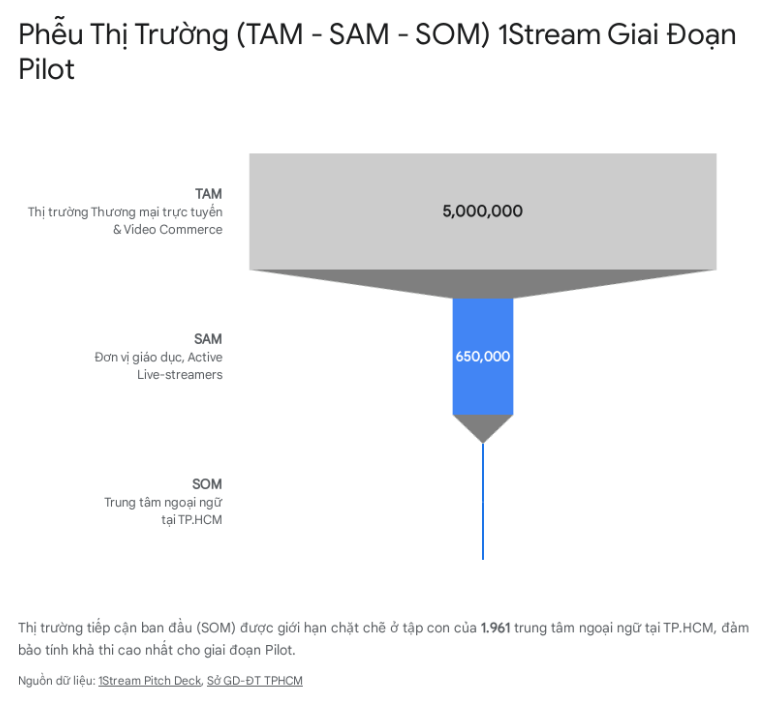
\includegraphics[width=0.85\linewidth]{imgs/PA3_pics/image1_v2.png}
    \caption{Mô hình phễu TAM -- SAM -- SOM cho 1Stream giai đoạn Pilot}
    \label{fig:tam-sam-som}
\end{figure}

\begin{WarningBox}[GIẢ ĐỊNH VỀ TỶ LỆ XUYÊN THẤU VÀ TẬP CON SOM]
Phân tích trên sử dụng con số 1.961 trung tâm\footnote{Nguồn: TPHCM: Khuyến khích mô hình câu lạc bộ của trung tâm ngoại ngữ, tin học (đã dẫn).} làm nền tảng SOM, đây là một điểm neo dữ liệu cứng đáng tin cậy. Tuy nhiên, lập luận cho rằng sẽ có \textbf{tối thiểu 15--20\%} trong tổng số các trung tâm này (tương đương khoảng 300 đến 400 trung tâm) sẽ thỏa mãn một cách hoàn hảo toàn bộ các bộ lọc nhận diện khắt khe (đội ngũ marketing chuẩn 3--5 người, chạy ads tích cực hàng ngày, có cấu trúc data khóa học chuẩn) hoàn toàn là một GIẢ ĐỊNH mang tính lạc quan. Đội ngũ Marketing của dự án không được phép tin tưởng tuyệt đối vào tỷ lệ này. Họ bị bắt buộc phải tiến hành thực thi các chiến dịch khai thác và cào dữ liệu kỹ thuật số (Data Scraping) một cách tinh vi, sử dụng các công cụ như Facebook Ads Library, để tiến hành kiểm chứng chéo và đo lường con số trung tâm thực tế đạt tiêu chuẩn trước khi quyết định ký duyệt giải ngân bất kỳ một khoản ngân sách quảng cáo lớn nào.
\end{WarningBox}

%% ================================================================
%% SECTION 5
%% ================================================================
\subsubsection{Nghệ thuật Tiếp cận Trinh sát số (Digital Reconnaissance) và Dẫn dắt Go-To-Market (GTM) qua Lăng kính Đánh giá Tiềm năng}

Phần phân tích này nhằm trả lời trực tiếp và sâu sát nhất cho bài toán cốt lõi: \textit{Làm thế nào để đội ngũ tiếp thị (Marketing) có thể nhận diện chính xác cái ICP cốt lõi đó giữa một thị trường bao la và hỗn loạn?} Chiến lược tiếp cận thị trường (GTM) trong giai đoạn Pilot của 1Stream không bao giờ được phép sa lầy vào tư duy mua các luồng lưu lượng truy cập giá rẻ hay chạy quảng cáo dàn trải trên diện rộng (Mass Marketing). Thay vào đó, chiến lược được định hình như một nghệ thuật ``săn lùng'' các tín hiệu số đặc thù (Digital Signals) và thực thi quy trình phân loại dữ liệu (Lead Qualification) cực đoan.

\paragraph{Cơ chế ``Săn'' ICP Cốt lõi trên không gian Digital (Digital Footprint Reconnaissance)}

Để phát hiện và nhận diện các trung tâm tiếng Anh hoặc tiếng Hàn hoàn hảo cho dự án, đội ngũ Marketing không thể áp dụng phương pháp gọi điện chào hàng lạnh (Cold Calling) một cách ngẫu nhiên từ danh bạ doanh nghiệp. Sự lãng phí thời gian vào các trung tâm không chạy quảng cáo số sẽ giết chết hiệu suất của bộ phận Sales. Thay vào đó, một quy trình nhận diện chủ động (Outbound Identification) dựa trên trí tình báo kỹ thuật số mã nguồn mở (OSINT) được thiết lập thông qua ba bước kỹ thuật sau:

Quy trình đầu tiên là thiết lập trạm quét tình báo thông qua Thư viện quảng cáo (Facebook Ads Library Recon). Chuyên viên tiếp thị của 1Stream sẽ sử dụng Facebook Ads Library, một công cụ minh bạch dữ liệu do Meta cung cấp\footnote{Nguồn: Facebook Ads là gì? Hướng dẫn chi tiết từ A -- Z -- CareerViet, truy cập ngày 16 tháng 7 năm 2026, \url{https://careerviet.vn/vi/talentcommunity/facebook-ads-la-gi-huong-dan-chi-tiet-tu-a-z.35A522A4.html}}, kết hợp với các bộ lọc từ khóa chuyên ngành được tối ưu hóa cao độ (ví dụ: ``Khóa học IELTS cam kết đầu ra'', ``Luyện thi TOPIK cấp tốc'', ``Ưu đãi học phí tiếng Anh tháng này'', ``Đăng ký test đầu vào miễn phí''). Khi quét hệ thống này, bất kỳ một Fanpage trung tâm nào duy trì việc chạy từ 5 chiến dịch quảng cáo mang tính chất chuyển đổi (Conversion Ads) trở lên cùng một lúc, đặc biệt nếu họ sử dụng các định dạng video ngắn dọc hoặc phát lại các đoạn cắt từ livestream (livestream replay), đều lập tức phát ra một tín hiệu số cực mạnh chứng minh họ ``đang chạy số'' quyết liệt. Phân tích tâm lý học kinh doanh cho thấy, các trung tâm này đang phải thiêu đốt một lượng ngân sách khổng lồ mỗi ngày và họ đang trong trạng thái khao khát đến tuyệt vọng việc tìm ra các phương pháp tối ưu hóa chỉ số CPL.\footnote{Nguồn: CHIẾN DỊCH QUẢNG CÁO KHÓA HỌC TIẾNG ANH TRÊN FACEBOOK VỚI NGÂN SÁCH 9.000.000Đ/THÁNG -- SPEAK NOW, truy cập ngày 16 tháng 7 năm 2026, \url{https://speaknow.vn/phu-kim-quy-chia-se-chien-dich-quang-cao-khoa-hoc-tieng-anh-tren-facebook/}} Sự xuất hiện của 1Stream lúc này chính là giải pháp dập tắt cơn đau tài chính đó.

Quy trình thứ hai là chiến dịch Giám sát Khung giờ vàng Livestream trên nền tảng TikTok (TikTok Live Monitoring). Đội ngũ sẽ triển khai các công cụ phân tích tự động hoặc phân công trực ban thủ công để rà quét các luồng phát sóng vào đúng khung giờ sinh tử từ 19h00 đến 22h30 mỗi tối.\footnote{Nguồn: GMV Max là gì? AI campaign đột phá của TikTok Shop 2026 | OneZ (đã dẫn).} Một tín hiệu nhận diện MQL (Marketing Qualified Lead) hoàn hảo nhất sẽ xuất hiện dưới hình thái sau: Khám phá ra một kênh TikTok của một trung tâm ngoại ngữ đang trong trạng thái phát sóng trực tiếp (LIVE), lượng người xem đồng thời (Concurrent Viewers -- CCV) duy trì ổn định nhưng không quá cao, dao động từ 30 đến 100 người. Tuy nhiên, tốc độ bình luận (comments per minute) từ khán giả diễn ra liên tục, nhưng người dẫn chương trình (Host) hoặc đội ngũ hỗ trợ phía sau lại có tốc độ phản hồi bằng văn bản quá chậm, liên tục đọc sót tên người dùng đang hỏi về thông tin khóa học. Khung cảnh hỗn loạn nhẹ này chính là biểu hiện vật lý rõ nét nhất của ``cường độ vấn đề'' (Pain Point) mà trung tâm đang gặp phải. Đây là cơ hội hoàn hảo để tác nhân AI Agent của 1Stream can thiệp, chứng minh khả năng phản hồi chính xác từng câu hỏi trong vòng vài giây mà không bao giờ biết mệt mỏi hay bỏ sót bất kỳ một khách hàng tiềm năng nào.

Quy trình thứ ba, mang tính quyết định trước khi thực hiện bước tiếp cận, là quá trình Đánh giá mức độ Chuẩn hóa Dữ liệu nội bộ (Data Readiness Check). Ngay sau khi phát hiện các tín hiệu mạnh từ hai bước trên, chuyên viên Marketing không được phép liên hệ ngay. Họ phải thực hiện một cuộc kiểm tra tĩnh bằng cách truy cập trực tiếp vào giao diện website chính thức hoặc cấu trúc trang đích (Landing Page) của trung tâm mục tiêu đó. Đích đến của cuộc kiểm tra là hệ thống phân cấp thông tin. Nếu trung tâm đó xây dựng một hệ thống Menu rõ ràng, sở hữu các trang con minh bạch về Báo giá (Pricing), Lịch khai giảng (Schedules) được cập nhật thường xuyên, và Hệ thống Câu hỏi Thường gặp (FAQ) đầy đủ -- thì luồng dữ liệu (Lead) này chính thức được đóng dấu ``Đủ điều kiện Data hoàn hảo''. Nó lập tức được đẩy thẳng xuống bước đánh giá sâu hơn, bởi hệ thống của họ đã sẵn sàng để trở thành cơ sở tri thức (Knowledge Base) huấn luyện cho AI của 1Stream mà không cần phải chỉnh sửa gì thêm.

\paragraph{Khái niệm lại Khung Phân loại Lead: Sự khác biệt giữa MQL và SQL trong Đặc thù ngành EdTech}

Để thiết lập một bức tường lửa bảo vệ thời gian của đội ngũ Sales, ngăn chặn tuyệt đối tình trạng gọi điện thoại nhầm đối tượng, quy trình chuyển đổi trạng thái vòng đời từ Marketing Qualified Lead (MQL) sang Sales Qualified Lead (SQL) phải được định nghĩa lại một cách căn bản cho phù hợp với những biến số đặc thù của ngành EdTech kết hợp SaaS. Tham chiếu các dữ liệu toàn cầu cho thấy, tỷ lệ chuyển đổi trung bình từ MQL sang SQL trong các doanh nghiệp cung cấp dịch vụ phần mềm B2B (B2B SaaS) thường duy trì ở mức khá cao, dao động ổn định trong khoảng từ 32\% đến 40\%.\footnote{Nguồn: B2B SaaS Conversion Rate Benchmarks 2026 by Funnel Stage, truy cập ngày 16 tháng 7 năm 2026, \url{https://konabayev.com/blog/b2b-saas-conversion-benchmarks-2026/}} Tỷ lệ này phản ánh một thị trường doanh nghiệp có tư duy hệ thống và chu kỳ mua sắm phần mềm rõ ràng. Tuy nhiên, khi áp dụng cùng một mô hình vào mảng giáo dục (EdTech) nói chung và các trung tâm ngoại ngữ nói riêng, tỷ lệ chuyển đổi này sụp đổ và rớt xuống một mức rất thấp, chỉ quanh quẩn ở ngưỡng 5\% đến 10\%.\footnote{Nguồn: How To: Turn MQLs into SQLs | EM360Tech, truy cập ngày 16 tháng 7 năm 2026, \url{https://em360tech.com/blog/mql-to-sql-guide}} Nguyên nhân của sự sụt giảm này xuất phát từ chu kỳ ra quyết định mua sắm của các giám đốc giáo dục thường bị kéo dài, sự dè dặt với các công nghệ AI mới, và tính chất phân mảnh cao của các cơ sở đào tạo quy mô nhỏ.

Đối mặt với thực trạng tỷ lệ chuyển đổi khắc nghiệt này, khung đánh giá năng lực tiềm năng của 1Stream được thiết lập vô cùng hà khắc và chia làm hai ranh giới phân định rõ ràng.

Ranh giới đầu tiên là việc định danh \textbf{MQL (Marketing Qualified Lead) -- Lead Đủ điều kiện Tiếp thị}. Để được công nhận là một MQL, hồ sơ đó phải là thông tin của một trung tâm ngoại ngữ đang hoạt động tại khu vực TP.HCM (tức là đã vượt qua thành công màng lọc vị trí địa lý của thị trường SOM). Hồ sơ này có thể do trung tâm tự nguyện để lại thông tin liên hệ, hoặc là kết quả do đội ngũ Marketing của 1Stream ``săn lùng'' thành công từ các chiến dịch trinh sát trên Facebook hay TikTok. Hơn thế nữa, MQL này bắt buộc phải thể hiện các hành vi số (Digital behavior) rõ nét, chẳng hạn như: có dữ liệu truy cập vào trang chủ của nền tảng 1Stream, nhấp chuột xem qua các trang giới thiệu tính năng lõi như ``AI Auto-Reply'', hoặc chủ động điền email công ty vào các biểu mẫu nhận bản tin. MQL là tín hiệu cho thấy sự quan tâm ban đầu, nhưng tuyệt đối chưa đủ độ chín để chuyển giao cho bộ phận bán hàng.

Ranh giới thứ hai, và cũng là giới hạn sinh tử, là việc thăng cấp lên \textbf{SQL (Sales Qualified Lead) -- Lead Đủ điều kiện Bán hàng}. Một MQL đang nằm trong hệ thống dữ liệu chỉ được phép thăng cấp và trao danh hiệu SQL khi và chỉ khi bộ phận Marketing đã thực hiện thành công bước xác minh chéo. Bước xác minh này thường được tiến hành qua một cuộc gọi sơ bộ đánh giá nhu cầu (Discovery call) hoặc một biểu mẫu khảo sát thông minh, nhằm đảm bảo MQL đó đáp ứng đồng thời ba tiêu chí bất khả kháng: Thứ nhất, họ xác nhận đội ngũ Marketing hoặc trực Live của họ hiện có quy mô chính xác từ 3 đến 5 nhân sự; Thứ hai, họ sở hữu và sẵn sàng cung cấp các tài liệu giáo trình và bảng giá dưới dạng dữ liệu tĩnh; Thứ ba, nhân sự mà 1Stream đang trao đổi phải là người có thực quyền ra quyết định cuối cùng (Decision Maker), hoặc chí ít là người bảo trợ dự án (Champion) có khả năng gây ảnh hưởng trực tiếp đến ngân sách mua sắm công cụ phần mềm của trung tâm. Bất kỳ sự thiếu hụt nào trong ba tiêu chí này đều khiến MQL bị giáng cấp. Chỉ những hồ sơ vượt qua khe cửa hẹp này, trở thành SQL thực thụ, mới được đặc cách chuyển giao cho đội ngũ Chuyên viên Phát triển Tài khoản cấp cao (Account Executive) để tiến hành dàn xếp các buổi trình diễn (demo) sản phẩm thực tế.

\begin{figure}[H]
    \centering
    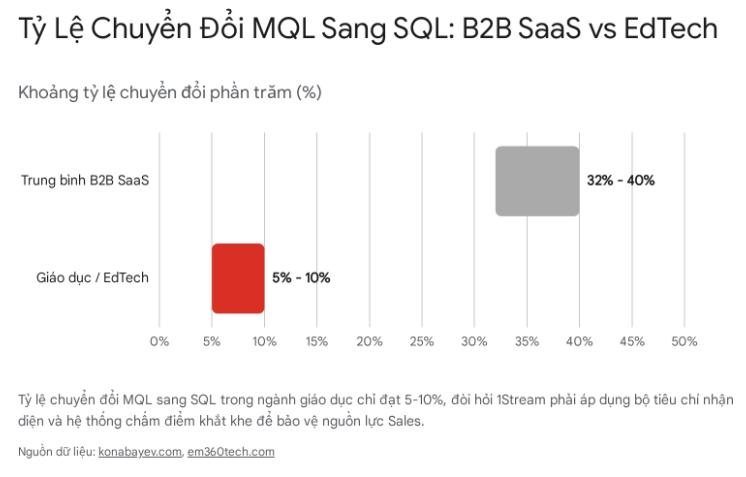
\includegraphics[width=0.85\linewidth]{imgs/PA3_pics/image2_v2.png}
    \caption{So sánh tỷ lệ chuyển đổi MQL-to-SQL giữa B2B SaaS và EdTech}
    \label{fig:mql-sql-comparison}
\end{figure}

%% ================================================================
%% SECTION 6
%% ================================================================
\subsubsection{Kiến trúc Hệ thống Chấm điểm Định lượng ICP (Lead Scoring Matrix) Dành cho Giai đoạn Pilot}

Quá trình chuyển hóa các đặc tính phân tích định tính về sự phù hợp của khách hàng từ các báo cáo phát triển sản phẩm (chương PA2) thành một công cụ định lượng sắc bén, có thể hoạt động độc lập trên hệ thống phần mềm thực chiến của đội ngũ Marketing, là bước đi bắt buộc. Để hiện thực hóa điều này, chúng tôi đã kiến tạo một Hệ thống chấm điểm đánh giá tiềm năng khách hàng (Lead Scoring Matrix) hoạt động dựa trên cơ chế trọng số tối đa là 100 điểm. Mọi tương tác, đặc điểm tổ chức và hành vi của một Khách hàng tiềm năng (Lead) đều sẽ được hệ thống theo dõi và cộng dồn điểm số. Khái niệm phân loại sẽ được tự động hóa hoàn toàn: chỉ những hồ sơ tích lũy vượt qua được ranh giới điểm quy định (Threshold) mới được quyền kích hoạt quy trình báo động chuyển đổi thành SQL.

\paragraph{Cấu trúc Thuật toán Thang điểm 100 và Bộ Tiêu chí Đánh giá}

Ma trận chấm điểm này không phân bổ điểm số đồng đều mà sử dụng nguyên tắc trọng số, trong đó những yếu tố quyết định khả năng áp dụng công nghệ AI ngay lập tức sẽ nắm giữ số điểm cao nhất.

\begin{table}[H]
    \centering
    \footnotesize
    \setlength{\tabcolsep}{3pt}
    \renewcommand{\arraystretch}{1.25}
    \caption{Ma trận chấm điểm đánh giá tiềm năng khách hàng (Lead Scoring Matrix) -- Thang 100 điểm}
    \label{tab:lead-scoring}
    \rowcolors{2}{paperBg}{white}
    \begin{tabularx}{\linewidth}{@{}L{0.14\linewidth}YL{0.08\linewidth}Y@{}}
        \toprule
        \rowcolor{softBlue}
        \textbf{Tiêu chí Đánh giá Cốt lõi (Core Criteria)} &
        \textbf{Diễn giải Cơ chế \& Quy trình Marketing thu thập tín hiệu} &
        \textbf{Phân bổ Trọng số} &
        \textbf{Khung Điểm Phạt (Negative / Penalty Logic)} \\ \midrule

        %% --- Row 1 ---
        \textbf{Cường độ vấn đề (Pain Point Intensity)} &

        Đo lường mức độ khủng hoảng trong vận hành hiện tại, đặc biệt là tình trạng quá tải bình luận và sự gia tăng mất kiểm soát của chi phí CPL.

        \textbf{Cơ chế thu thập:} Các kỹ thuật viên Marketing phát hiện trung tâm có tỷ lệ rớt bình luận cao trên livestream TikTok, hoặc đang đổ tiền chạy quảng cáo liên tục trên FB Ads Library nhưng hệ thống Landing Page lại hoàn toàn vắng bóng các công cụ phản hồi tự động (chatbots) ban đầu. &

        \textbf{20 điểm} &

        $-20$ điểm (Áp dụng ngay lập tức nếu dữ liệu cho thấy livestream của trung tâm có lượng người xem bằng 0 hoặc trung tâm không hề triển khai bất kỳ chiến dịch quảng cáo trả phí nào trong vòng 30 ngày qua). \\ \midrule

        %% --- Row 2 ---
        \textbf{Sự tương thích về quy mô nguồn lực (Marketing Team Size)} &

        Đánh giá tính lý tưởng của cấu trúc nhân sự, hướng tới điểm ngọt từ 3 đến 5 người.

        \textbf{Cơ chế thu thập:} Chuyên viên thực hiện các nghiệp vụ tra cứu thông tin tình báo doanh nghiệp thông qua mạng lưới LinkedIn, hoặc theo dõi các cổng thông tin việc làm (như Ybox, CareerViet) để xem trung tâm có đang trong tình trạng đăng tin tuyển dụng khẩn cấp các vị trí chuyên viên Facebook Ads hay Livestreamer ca tối hay không.\footnote{Nguồn: [Online] Trung Tâm Tiếng Anh IGEMS Tuyển Dụng Thực Tập Sinh Dạy Tiếng Anh -- Livestream Full-time 2025 -- YBOX (đã dẫn).} &

        \textbf{15 điểm} &

        0 điểm (Hệ thống không cộng điểm nếu quy mô đội ngũ quá manh mún dưới 2 người, hoặc cấu trúc đã phình to quá phức tạp trên 10 người). \\ \midrule

        %% --- Row 3 ---
        \textbf{Mật độ và Tần suất sử dụng (Usage Frequency)} &

        Xác nhận thói quen duy trì các phiên phát sóng trực tiếp một cách đều đặn vào các khung giờ vàng buổi tối (19h00--22h30). Đi kèm với đó là nhu cầu hiển nhiên về việc sản xuất các đoạn video ngắn hàng ngày để duy trì tương tác. &

        \textbf{15 điểm} &

        $-10$ điểm (Trừ điểm mạnh nếu hồ sơ chỉ ra rằng trung tâm chỉ duy trì lịch livestream mang tính sự kiện, ví dụ 1 tháng chỉ tổ chức 1 lần). \\ \midrule

        %% --- Row 4 ---
        \textbf{Mức độ chuẩn hóa của Khối Dữ liệu tĩnh (Data Standardization)} &

        Kiểm định khả năng cung cấp nền tảng tri thức cho AI, thông qua việc có sẵn các bảng giá cố định và lộ trình học mang tính chất tĩnh.

        \textbf{Cơ chế thu thập:} Bot thu thập hoặc chuyên viên truy cập trực tiếp website của trung tâm, nếu hệ thống điều hướng (menu) có chứa các thư mục công khai như ``Học phí'', ``Lịch khai giảng'', hồ sơ lập tức đạt điểm tối đa ở hạng mục này. &

        \textbf{15 điểm} &

        $-20$ điểm (Phạt nặng nếu hệ thống phát hiện chính sách tiếp thị của trung tâm là ``Inbox để nhận báo giá bí mật'', khiến AI không có cơ sở dữ liệu để vận hành). \\ \midrule

        %% --- Row 5 ---
        \textbf{Năng lực chi trả và Dòng tiền tiếp thị (Willingness to Pay)} &

        Phân tích tiềm lực tài chính dựa trên bằng chứng về việc có phân bổ ngân sách Marketing rõ ràng. Các ước tính vĩ mô chỉ ra rằng những trung tâm duy trì chạy ads liên tục sẽ phải gánh CPL trung bình 24.584 VNĐ và sở hữu một ngân sách duy trì dài hạn.\footnote{Nguồn: Chạy quảng cáo Facebook bao nhiêu tiền cập nhật mới nhất | On Digitals -- Ondigitals (đã dẫn).} Sự sẵn sàng đầu tư này chứng minh họ đủ sức chi trả cho các gói thuê bao của một công cụ SaaS. &

        \textbf{15 điểm} &

        0 điểm (Áp dụng cho các mô hình dự án sinh viên khởi nghiệp phi lợi nhuận, hoặc các trung tâm hoạt động cộng đồng miễn phí không có nhu cầu tối ưu hóa lợi nhuận). \\ \midrule

        %% --- Row 6 ---
        \textbf{Khả năng Tích hợp Độc lập (Tech Fit / No Complex API)} &

        Đánh giá mức độ sẵn lòng chấp nhận sử dụng giao diện bảng điều khiển (dashboard) độc lập của 1Stream, thay vì đưa ra các yêu sách đòi hỏi đội ngũ kỹ thuật phải viết mã kết nối API cắm sâu vào hệ thống ERP cồng kềnh của tập đoàn. &

        \textbf{10 điểm} &

        $-50$ điểm (Đây là án phạt mang tính chất vô hiệu hóa hồ sơ, áp dụng khi khách hàng khăng khăng đòi hỏi các giao thức kết nối API phức tạp ngay trong tháng chạy Pilot). \\ \midrule

        %% --- Row 7 ---
        \textbf{Rào cản Tính hợp pháp (Pháp lý sinh trắc học)} &

        Xác nhận tuyệt đối quyền sở hữu bản quyền hợp pháp đối với hình ảnh và đặc điểm giọng nói của nhân sự sẽ được sử dụng làm nguồn để huấn luyện AI. (Yếu tố này thường được đánh giá trực tiếp qua khảo sát đầu vào trong cuộc gọi Discovery Call). &

        \textbf{10 điểm} &

        \textbf{LOẠI TRỰC TIẾP} (Nếu khách hàng bộc lộ sự mập mờ hoặc không chứng minh được tính pháp lý, toàn bộ hồ sơ lập tức bị đóng băng bất kể tổng điểm các phần khác cao đến đâu). \\ \midrule

        %% --- Row TOTAL ---
        \textbf{TỔNG KIỂM SOÁT TỐI ĐA} & & \textbf{100 điểm} & \\

        \bottomrule
    \end{tabularx}
    \rowcolors{2}{}{}
\end{table}

\paragraph{Thuật toán Ngưỡng Phân loại và Quy trình Chuyển giao (Threshold Handoff Rules)}

Được vận hành trên nền tảng của cấu trúc tính điểm chi tiết ở trên, luồng làm việc tự động (Automated Workflow) giữa bộ phận Marketing thu thập dữ liệu và bộ phận Sales chốt hợp đồng sẽ được vận hành một cách trơn tru, lạnh lùng và không có chỗ cho cảm tính cá nhân, cụ thể như sau:

Cấp độ đầu tiên, áp dụng cho dải điểm \textbf{Từ 0 đến 45 Điểm}: Những hồ sơ rơi vào vùng trũng này sẽ ngay lập tức được hệ thống gán nhãn là ``Cold Lead'' (Lead lạnh) hoặc ``Nurture'' (Cần nuôi dưỡng). Về cơ bản, đây chính là nhóm khách hàng thuộc Phân khúc liền kề (Adjacent Segment) hoặc nhóm Chưa ưu tiên do thiếu hụt ngân sách hoặc chưa sẵn sàng về mặt dữ liệu. Đội ngũ Marketing sẽ tự động đưa các liên hệ này vào một phễu gửi Email tự động dài hạn nhằm mục đích giáo dục thị trường, cập nhật các tính năng mới hoặc gửi các báo cáo ngành. Tại dải điểm này, hoàn toàn không có sự tham gia của bất kỳ nhân sự Sales nào để tránh lãng phí thời gian.

Cấp độ thứ hai, áp dụng cho dải điểm \textbf{Từ 46 đến 74 Điểm}: Các hồ sơ vượt qua ngưỡng 45 điểm sẽ chính thức được thăng cấp vào nhóm MQL. Trạng thái này kích hoạt một nhiệm vụ cho đội ngũ phát triển kinh doanh vòng ngoài (như Telesales hoặc Sales Development Representative -- SDR). Họ sẽ có nhiệm vụ thực hiện một cuộc gọi điện thoại sơ bộ (Discovery Call), được khống chế nghiêm ngặt không quá 5 phút. Mục tiêu duy nhất của cuộc gọi này là để xác thực các giả định mà hệ thống chấm điểm đã gán, đặc biệt xoáy sâu vào việc xác minh lại Cường độ vấn đề đang gặp phải và Mức độ chuẩn hóa của dữ liệu nội bộ.

Cấp độ thứ ba, cấp độ tối cao, áp dụng cho dải điểm \textbf{Từ 75 đến 100 Điểm}: Bất kỳ hồ sơ nào lọt vào dải điểm này sẽ chính thức rũ bỏ mọi sự nghi ngờ để trở thành một \textbf{Core ICP (SQL)} hoàn hảo. Lúc này, hệ thống sẽ tự động kích hoạt lệnh chuyển thẳng Lead đó vào hệ thống Quản trị Quan hệ Khách hàng (CRM) nội bộ, đồng thời phân công trực tiếp cho các Chuyên viên Phát triển Tài khoản cấp cao (Account Executive). Đây là những bức chân dung của một trung tâm ngoại ngữ lý tưởng: họ có một đội ngũ 4 người đang kiệt sức, họ đang thiêu đốt hàng chục triệu đồng để chạy quảng cáo Facebook mỗi tháng\footnote{Nguồn: Facebook Ads Cho Giáo Dục: Checklist Hoàn Chỉnh (2026) -- NgoiSaoMedia (đã dẫn).}, họ liên tục tổ chức livestream bất chấp lượng người xem đôi khi khiêm tốn, họ có bảng giá công khai minh bạch rõ như ban ngày, và quan trọng nhất, họ đang bị ``ngộp thở'' trong vòng xoáy của việc phải phản hồi hàng trăm bình luận một cách thủ công. Nhiệm vụ của đội ngũ Sales lúc này không còn là ``thuyết phục'' họ sử dụng phần mềm, mà là hành động như những vị cứu tinh: Sales sẽ ưu tiên tối đa việc thiết lập ngay các buổi trình diễn tính năng (Demo) trực tiếp -- có thể qua các nền tảng trực tuyến hoặc ưu tiên gặp mặt trực tiếp (Offline) tại trụ sở trung tâm ở TP.HCM -- và ngay lập tức đưa ra đề xuất chốt hợp đồng đối với Gói dịch vụ 30 giờ/kênh của nền tảng 1Stream.

\begin{WarningBox}[GIẢ ĐỊNH VỀ TÍNH CHÍNH XÁC CỦA HỆ THỐNG CHẤM ĐIỂM TỰ ĐỘNG BẰNG OSINT]
Cơ chế vận hành của quy trình đánh giá các tiêu chí mang tính định lượng như ``Tần suất sử dụng'' và đặc biệt là ``Mức độ chuẩn hóa Data'' hiện tại đang được xây dựng trên một giả định cốt lõi: Các kỹ thuật viên Marketing của dự án, hoặc các hệ thống thu thập dữ liệu tự động, có khả năng trích xuất đầy đủ các thông tin công khai (Open-Source Intelligence -- OSINT) trên môi trường Internet mà không tốn quá nhiều thời gian quét thủ công. Tuy nhiên, rủi ro sai lệch xuất hiện nếu thiết kế Website của khách hàng cố tình ẩn giấu cấu trúc dữ liệu đào tạo (bảng giá, lịch học) đằng sau một bức tường biểu mẫu đăng ký (gated content) buộc người dùng phải điền thông tin mới được xem. Trong trường hợp này, điểm số đánh giá sẽ bị đánh tụt một cách oan uổng. Để giải quyết rủi ro này, quy trình vận hành bắt buộc phải kết hợp sử dụng các biểu mẫu thu thập thông tin hấp dẫn (Lead Magnet Form) chứa các bảng câu hỏi yêu cầu chính các chủ trung tâm phải tự đánh giá hiện trạng của họ (Self-assess), từ đó lấy dữ liệu chủ quan này để đối chiếu chéo với dữ liệu khách quan thu thập được, đảm bảo tính chính xác tuyệt đối trước khi ra quyết định phân loại Lead.
\end{WarningBox}

%% ================================================================
%% SECTION 7
%% ================================================================
\subsubsection{Khuyến nghị Triển khai Chiến lược Tối ưu hóa Hành trình Khách hàng}

Việc đưa ra quyết định chiến lược đóng gói toàn bộ giá trị công nghệ phức tạp của 1Stream thành một Gói sản phẩm tiêu chuẩn 30 giờ/kênh, đồng thời nhắm mục tiêu một cách cực đoan vào một ngách thị trường cụ thể là các trung tâm ngoại ngữ có trụ sở tại TP.HCM, là một nước đi chiến lược cực kỳ sắc bén (Laser-focused strategy). Thay vì rơi vào cái bẫy ảo tưởng của việc cố gắng bán một giải pháp chung chung cho hàng triệu người bán hàng trên mạng xã hội -- một nỗ lực thường dẫn đến sự pha loãng định vị thương hiệu và cạn kiệt dòng tiền -- việc dồn toàn lực tập trung vào các trung tâm đào tạo IELTS hay TOEIC có quy mô vận hành nhỏ giúp sản phẩm kiểm chứng (validate) được cốt lõi công nghệ AI của mình một cách an toàn, nhanh chóng và có khả năng thu hồi vốn, đồng thời vẫn bảo vệ được nguồn lực giới hạn của đội ngũ R\&D.

Để các hoạt động tiếp thị (Marketing) thực sự nhận diện được chính xác cái ICP cốt lõi đang lẩn khuất trên thị trường một cách hiệu quả nhất, ba nhóm hành động chiến thuật mang tính mệnh lệnh dưới đây bắt buộc phải được triển khai trên thực địa ngay lập tức, không có bất kỳ sự nhân nhượng nào:

Hành động thứ nhất đòi hỏi một sự thay đổi tư duy triệt để trong việc phân bổ ngân sách: \textbf{Chấm dứt vô điều kiện mọi chiến dịch quảng cáo diện rộng mang tính chất ``Mass Ads''.} Đội ngũ tiếp thị phải ngay lập tức ngừng việc đổ tiền vào các chiến dịch quảng cáo hiển thị rộng rãi, nhắm mục tiêu vào các từ khóa mơ hồ mang tính chất khái quát cao như ``Giải pháp livestream toàn diện'' hay ``Phần mềm tăng đơn hàng''. Toàn bộ ngân sách giải phóng được từ đây phải được chuyển hướng và tái cấu trúc hoàn toàn sang các mô hình tiếp thị có độ chính xác cao hơn, cụ thể là Tiếp thị thu hút (Inbound Marketing) và đặc biệt là mô hình Tiếp thị Dựa trên Tài khoản (Account-Based Marketing -- ABM). Mục tiêu của các chiến dịch này không phải là đám đông, mà được thiết kế như những mũi tên bắn thẳng tới các cá nhân nắm giữ các chức danh cụ thể như ``Giám đốc trung tâm đào tạo'', ``Founder học viện ngoại ngữ'', hay ``Trưởng phòng Marketing Giáo dục'', và phải giới hạn khu vực phân phối quảng cáo bằng hàng rào địa lý (geo-fencing) nằm gọn trong ranh giới TP.HCM.

Hành động thứ hai định hình lại thông điệp truyền thông: \textbf{Sử dụng chính ``Nỗi đau CPL'' của khách hàng làm mồi nhử chết người (Lead Magnet).} Phân tích của các chuyên gia trong ngành đã chỉ ra một sự thật phũ phàng: chi phí CPL cho ngành giáo dục, dù trên lý thuyết các báo cáo thường được tô vẽ ở mức thấp (quanh ngưỡng 24.000 VNĐ)\footnote{Nguồn: Chạy quảng cáo Facebook bao nhiêu tiền cập nhật mới nhất | On Digitals -- Ondigitals (đã dẫn).}, nhưng trong môi trường thực chiến chạy Facebook Ads với sự cạnh tranh đẫm máu, mức chi phí này hoàn toàn có thể vọt lên tới nửa triệu đồng (500.000 VNĐ) cho một Lead.\footnote{Nguồn: Facebook Ads Cho Giáo Dục: Checklist Hoàn Chỉnh (2026) -- NgoiSaoMedia (đã dẫn).} Nguyên nhân chủ đạo của sự lãng phí này là tỷ lệ thoát trang (bounce rate) và sự rời bỏ của khách hàng do tốc độ phản hồi tin nhắn của trung tâm quá chậm chạp. Thông điệp Marketing của 1Stream không được phép nói về các thuật ngữ kỹ thuật khô khan của AI. Thông điệp phải đâm thẳng vào nỗi sợ hãi tài chính của chủ doanh nghiệp: \textit{``AI Agent của nền tảng chúng tôi sẽ đứng gác và giữ chân từng học viên của bạn lúc 22h00 đêm, ngay cả khi toàn bộ đội ngũ tư vấn của bạn đã đi ngủ. Chúng tôi cam kết chặn đứng sự rò rỉ ngân sách và ép CPL của bạn giảm xuống 3 lần''}. Bằng chứng thực nghiệm luôn cho thấy, các thông điệp đánh trực diện vào hiệu quả tài chính và nỗi sợ mất tiền luôn mang lại tỷ lệ chuyển đổi từ dữ liệu thô sang SQL cao nhất trong mọi chiến dịch tiếp thị B2B.

Hành động thứ ba, và là hành động khó khăn nhất về mặt tâm lý đối với đội ngũ bán hàng: \textbf{Thiết lập kỷ luật Tôn trọng Tiêu chí Loại trừ một cách tuyệt đối (Zero Tolerance Policy).} Ban giám đốc dự án không được phép thỏa hiệp, không được phép bẻ cong nguyên tắc để tiếp nhận bất kỳ một khách hàng nào không chứng minh được họ có hệ thống dữ liệu tĩnh rõ ràng, hoặc những khách hàng khăng khăng đưa ra yêu sách tích hợp API rườm rà. Phải thấm nhuần tư tưởng rằng, mục tiêu tối thượng của giai đoạn Pilot không phải là chạy theo doanh thu tối đa bằng mọi giá, mà là chứng minh được tính khả thi của năng lực kỹ thuật cốt lõi và kiến tạo nên những Câu chuyện thành công (Case Study) mang tính đại diện hoàn hảo. Việc cố gắng nuông chiều và chốt một hợp đồng từ một Enterprise Lead (Khách hàng doanh nghiệp lớn) ngay trong giai đoạn Pilot, với hy vọng vào một khoản doanh thu lớn, thực chất là một liều thuốc độc. Nó sẽ bào mòn đến kiệt quệ nguồn lực vốn đã ít ỏi của đội ngũ kỹ thuật, làm trễ nải tiến độ hoàn thiện phiên bản sản phẩm thương mại (MVP), và cuối cùng có thể đánh sập toàn bộ cấu trúc kiến trúc phần mềm vì phải chắp vá để phục vụ một hệ thống quá tầm kiểm soát.

Chiến lược phân khúc khách hàng chuyên sâu và kế hoạch tiếp cận thị trường (GTM) này không phải là những ý tưởng lý thuyết suông. Nó được xây dựng và đúc kết trên sự thấu hiểu sâu sắc không chỉ về kiến trúc sản phẩm của 1Stream, mà quan trọng hơn là sự thấu hiểu về bản chất tàn khốc và sự khắc nghiệt trong hệ sinh thái cạnh tranh của ngành Giáo dục -- Ngoại ngữ hiện đại. Việc tuân thủ một cách tuyệt đối và kỷ luật đối với khung phân khúc thị trường đã được thiết lập này không chỉ là một khuyến nghị, mà sẽ là yếu tố duy nhất quyết định sinh mệnh và quỹ đạo thành công của dự án 1Stream trong giai đoạn thương mại hóa đầu tiên.

%% ================================================================
%% WORKS CITED / DANH MỤC NGUỒN THAM KHẢO
%% (Tất cả các nguồn đã được chuyển thành \footnote trong bản văn)
%% ================================================================
% [1]  Giáo dục trực tuyến edtech, elearning, đào tạo trực tuyến. đào tạo Online, accessed July 16, 2026, https://www.nguyentrihien.com/
% [2]  Báo cáo thị trường EdTech & eLearning Vietnam 2026 | PDF -- Slideshare, accessed July 16, 2026, https://www.slideshare.net/slideshow/bao-cao-th-tr-ng-edtech-elearning-vietnam-2026/286243550
% [3]  TPHCM: Khuyến khích mô hình câu lạc bộ của trung tâm ngoại ngữ, tin học, accessed July 16, 2026, https://gdthuongxuyen.hcm.edu.vn/tin-hoat-dong/tphcm-khuyen-khich-mo-hinh-cau-lac-bo-cua-trung-tam-ngoai-ngu-tin-hoc/ctmb/42180/82845
% [4]  TPHCM có 1.961 trung tâm ngoại ngữ, tin học, nhiều nơi quảng cáo sai sự thật, accessed July 16, 2026, https://laodong.vn/giao-duc/tphcm-co-1961-trung-tam-ngoai-ngu-tin-hoc-nhieu-noi-quang-cao-sai-su-that-1580712.ldo
% [5]  Trung tâm ngoại ngữ Hoàng Việt 6 năm liền nhận Giấy khen từ Sở GD&ĐT TP.HCM, accessed July 16, 2026, https://tuoitre.vn/khoahocphothong/trung-tam-ngoai-ngu-hoang-viet-6-nam-lien-nhan-giay-khen-tu-so-gd-dt-tp-hcm-261421.html
% [6]  Gần 2.000 trung tâm ngoại ngữ, tin học được cấp phép: Một số nơi quảng cáo sai sự thật, accessed July 16, 2026, https://tuoitre.vn/plo/gan-2000-trung-tam-ngoai-ngu-tin-hoc-duoc-cap-phep-mot-so-noi-quang-cao-sai-su-that-post872241.html
% [7]  Chạy quảng cáo Facebook bao nhiêu tiền cập nhật mới nhất | On Digitals -- Ondigitals, accessed July 16, 2026, https://ondigitals.com/vi/chay-quang-cao-facebook-bao-nhieu-tien/
% [8]  Tất tần tật về phí quảng cáo Facebook bạn nên biết -- BurgerPrints, accessed July 16, 2026, https://burgerprints.com/vi/phi-quang-cao-facebook/
% [9]  Facebook Ads Cho Giáo Dục: Checklist Hoàn Chỉnh (2026) -- NgoiSaoMedia, accessed July 16, 2026, https://ngoisaomedia.net/bai-viet/facebook-ads-cho-giao-duc-checklist-hoan-chinh-2026-1780978680408-9hta1/
% [10] Hàng nghìn phụ huynh yêu cầu hoàn trả học phí, TP. HCM dự kiến đình chỉ các trung tâm Apax Leaders -- VietnamFinance, accessed July 16, 2026, https://vietnamfinance.vn/hang-nghin-phu-huynh-yeu-cau-hoan-tra-hoc-phi-tp-hcm-du-kien-dinh-chi-cac-trung-tam-apax-leaders-d94889.html
% [11] TP HCM: Giải thể 20 trung tâm Anh ngữ Apax Leaders, accessed July 16, 2026, https://giaoducthudo.giaoducthoidai.vn/tp-hcm-giai-the-20-trung-tam-anh-ngu-apax-leaders-139178.html
% [12] [CSH2026][1Stream][FINAL PITCH DECK].pdf
% [13] GMV Max là gì? AI campaign đột phá của TikTok Shop 2026 | OneZ, accessed July 16, 2026, https://onezdigital.vn/blog/gmv-max-tiktok-shop-la-gi-2026
% [14] [Online] Trung Tâm Tiếng Anh IGEMS Tuyển Dụng Thực Tập Sinh Dạy Tiếng Anh -- Livestream Full-time 2025 -- YBOX, accessed July 16, 2026, https://ybox.vn/tuyen-dung/online-trung-tam-tieng-anh-igems-tuyen-dung-thuc-tap-sinh-day-tieng-anh-full-time-2025-67dd13aff49350455812bb8e
% [15] Học Tiếng Hàn Giao Tiếp Hiệu Quả -- Trung Tâm Ngoại Ngữ LingGo, accessed July 16, 2026, https://linggo.edu.vn/trung-tam-tieng-han-linggo-hoc-tieng-han-giao-tiep-hieu-qua/
% [16] Facebook Ads là gì? Hướng dẫn chi tiết từ A -- Z -- CareerViet, accessed July 16, 2026, https://careerviet.vn/vi/talentcommunity/facebook-ads-la-gi-huong-dan-chi-tiet-tu-a-z.35A522A4.html
% [17] 5 Bước Để Chạy Quảng Cáo Facebook Ads Cho Trung Tâm Ngoại Ngữ, accessed July 16, 2026, https://vietnamteachingjobs.com/blog/5-buoc-de-chay-facebook-ads-cho-trung-tam-ngoai-ngu/
% [18] CHIẾN DỊCH QUẢNG CÁO KHÓA HỌC TIẾNG ANH TRÊN FACEBOOK VỚI NGÂN SÁCH 9.000.000Đ/THÁNG -- SPEAK NOW, accessed July 16, 2026, https://speaknow.vn/phu-kim-quy-chia-se-chien-dich-quang-cao-khoa-hoc-tieng-anh-tren-facebook/
% [19] CPL là gì? Cách tính CPL (Cost per lead) & tối ưu quảng cáo CPL -- MISA AMIS, accessed July 16, 2026, https://amis.misa.vn/59497/cpl-la-gi/
% [20] B2B SaaS Conversion Rate Benchmarks 2026 by Funnel Stage, accessed July 16, 2026, https://konabayev.com/blog/b2b-saas-conversion-benchmarks-2026/
% [21] How To: Turn MQLs into SQLs | EM360Tech, accessed July 16, 2026, https://em360tech.com/blog/mql-to-sql-guide
% [22] Lead là gì? Các bước tạo lead dễ áp dụng cho người mới bắt đầu -- Vieclam24h, accessed July 16, 2026, https://vieclam24h.vn/nghe-nghiep/tram-sac-ky-nang/lead-la-gi
